\textbf{ID:} UC15 (Manage Displayed Posts) \\
\textbf{Scope:} CS Automated Information Timeline \\
\textbf{Level:} User goal \\
\textbf{Primary Actor:} Office Manager \\
\textbf{Stakeholders and Interests:}
\begin{itemize}
    \item Admin/Reviewer: Wants to ensure a curated set of posts are displayed for guests
    \item Guest/Audience: Wants to be able to see priority posts from the department
    \item Faculty: Wants to ensure their relevant/priority posts are displayed to guests
\end{itemize}
\textbf{Preconditions:}
\begin{itemize}
    \item User with Office Manager role has been authenticated
    \item More than 10 posts exist in the system to allow assigning of priority
\end{itemize}
\textbf{Postconditions:}
\begin{itemize}
    \item Curated list of posts are displayed on the TV display
    \item The ordering of displayed posts is correct
\end{itemize}
\textbf{Main Success Scenario:}
\begin{enumerate}
    \item User navigates to view all posts
    \item System displays all posts
    \item User selects post to be displayed on the main TV display
    \item The system presents the current list of curated posts
    \item Repeat step 3 and 4 until all desired posts are selected by the user
    \item System presents final list of posts to be displayed on the main display
    \item User approves final list of media
    \item The system records the final list and the user ID associated with the created list
    \item The system updates the main display with the curated list of posts
    \item The main display begins to display the new posts
    \item The system notifies the user that the list is being displayed
\end{enumerate}
\textbf{Alternative Flows:} \\
3A: User does not deem any posts need to be displayed
\begin{enumerate}
    \item User decides to not provide a list based on the currently available media
    \item The user exits the action of curating the displayed posts
    \item The system discards any in work lists
\end{enumerate}
3B: The user wishes to change a previously selected post
\begin{enumerate}
    \item User selects post to not be displayed
    \item The system updates the list of curated posts
    \item Renter at beginning of step 3
\end{enumerate}
7A: The user needs to change the order of curated list
\begin{enumerate}
    \item The user selects the post they wish to change position
    \item The user indicates which position the post should be displayed in
    \item The system updates the curated list
    \item The system re-presents the final list to user for approval
    \item Renter at step 7 entry
\end{enumerate}

\begin{figure}[H]
    \centering
    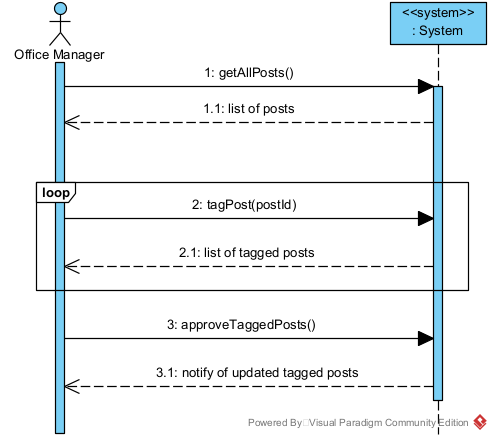
\includegraphics[width=0.8\textwidth]{images/SSD-UC15-ManageDisplayedPosts.png}
    \centering
    \caption{System Sequence Diagram: Manage Displayed Posts}
\end{figure}

\textbf{Operation:} getAllPosts() \\
\textbf{Cross-References:} UC15 (Manage Displayed Posts) \\
\textbf{Pre-conditions:}
\begin{itemize}
    \item Posts exist in system
    \item Post count $>$ 10
\end{itemize}
\textbf{Post-conditions:}
\begin{itemize}
    \item All posts returned to user (create list of posts, \emph{lp})
\end{itemize}

\textbf{Operation:} tagPost(postId) \\
\textbf{Cross-References:} UC15 (Manage Displayed Posts) \\
\textbf{Pre-conditions: }
\begin{itemize}
    \item Size of \emph{lp} $<$ 10
\end{itemize}
Post-conditions:
\begin{itemize}
    \item Post item, \emph{p}, is added to \emph{lp}
    \item Size of \emph{lp} $\leq$ 10
\end{itemize}

\textbf{Operation:} approveTaggedPosts() \\
\textbf{Cross-References:} UC15 (Manage Displayed Posts) \\
\textbf{Pre-conditions:}
\begin{itemize}
    \item Size of \emph{lp} = 10
    \item \emph{lp} has not been approved
\end{itemize}
\textbf{Post-conditions:}
\begin{itemize}
    \item \emph{lp} is approved
    \item MainDisplay updates with contents of \emph{lp}
\end{itemize}